\documentclass[12pt]{article}
\usepackage[letterpaper, margin=1in]{geometry}
\usepackage[dvipsnames]{xcolor}
\usepackage{graphicx}
\usepackage{caption}
\graphicspath{{./figures/}}
\usepackage{hyperref}
\hypersetup{
    colorlinks=true,   
    urlcolor=blue,
}
\usepackage{parskip}
\usepackage{amsmath}
\usepackage{siunitx}
\usepackage{pgfplots}
\usepackage{pgfplotstable}
\pgfplotsset{compat = newest}
\usepackage{titlesec}
\usepackage{listings}
\usepackage{lstautogobble}
\usepackage[framed, numbered]{matlab-prettifier}

\definecolor{backgroundColour}{rgb}{0.95,0.95,0.92}
\lstset{
    frame=single,
    breaklines=true,
    numbers=left,
    tabsize=4,
    backgroundcolor=\color{backgroundColour},
    keywordstyle=\color{red},
    identifierstyle=\color{blue},
    commentstyle=\color{gray}}

\titleformat*{\section}{\large\bfseries}
%\allowdisplaybreaks

% remove vertical spacing above top figure
\makeatletter
\setlength{\@fptop}{0pt}
\makeatother
%

\title{COMPENG 4DK4 Lab 4 Report}
\author{
    Aaron Pinto \\
    pintoa9 \\
    %L02
    \and
    Raeed Hassan \\
    hassam41 \\
    %L02
}

\begin{document}

\maketitle
\clearpage

\section*{Random Number Generator Seeds}
For the experiments in this lab, we used the same set of 8 random number seeds for all experiments. Experiment 1 instructs us to include runs with our \textit{McMaster Student ID numbers} as our seeds. We used our \textit{McMaster IDs} and shifted them by one digit at a time to create 4 different seeds from each our IDs, for a total of 8 different seeds. All the random number generator seeds can be seen in Table~\ref{tab:random_seeds}. In the C code used for the experiments, leading zeroes are removed.

\begin{table}[h]
	\centering
	\begin{tabular}{|l|l|}
	\hline
	400188200 & 400190637 \\ \hline
	001882004 & 001906374 \\ \hline
	018820040 & 019063740 \\ \hline
	188200400 & 190637400 \\ \hline
	\end{tabular}
\caption{Random Number Generator Seeds}
\label{tab:random_seeds}
\end{table}

\section*{Experiment 2}
% Using the provided simulation code, generate a set of curves that show the tradeoffs between blocking probability, offered load (in Erlangs) and the number of channels. (Curves of this kind were presented earlier in class. See the “Circuit Switching Performance” lecture overheads.) Compare your results to that obtained using the Erlang B formula. According to Erlang B, the probability that a call is blocked is given by
% PB = AN /N ! ∑N i=0 Ai/i!
% where A is the offered load (in Erlangs) and is given by
% A = λh
% where λ is the call arrival rate (in calls per unit time, e.g., calls/minute), h is the average call holding time (in the same time units, e.g., minutes), and N is the total number of channels. Write a program to perform this computation (Feel free to use any programming language you want, e.g., Matlab, C, etc.) Include a listing of your program in your writeup. Check the results of your program using one of many online Erlang B calculators. Just google search for “Erlang B calculator”. Include the URL of the calculator that you used. The set of curves that show the tradeoffs between blocking probability, offered load (in Erlangs) and the number of channels can be seen in Figure~\ref{fig:exp2}. We can observe that the blocking probability decreases as the number of channels increase, and increasing the offered load will increase the blocking probability at a given number of channels.
The set of curves that show the tradeoffs between blocking probability, offered load (in Erlangs) and the number of channels can be seen in Figure~\ref{fig:exp2}. We can observe that the blocking probability decreases as the number of channels increase, and increasing the offered load will increase the blocking probability at a given number of channels.

When plotting these results with the Erlang B formula in MATLAB, we observe the same results with essentially identical curves as seen in Figure~\ref{fig:exp2_matlab}. The MATLAB code used to calculate the Erlang B formula can be seen in Listing~\ref{list:exp2}. We compared several of our results of from our program with an \href{https://owenduffy.net/traffic/erlangb.htm}{online Erlang B calculator} and had matching results. For example, for $A = 5, N = 10$, both calculated $P_B = 0.184$. 

\begin{lstlisting}[style=Matlab-editor,firstnumber=3,caption=Erlang B Formula, label=list:exp2]
syms k

for A = 1:20
	for N = 1:20
		PB(A,N) = ((A^N)/factorial(N))/symsum(A^k/factorial(k),k,0,N);
	end
end
\end{lstlisting}

\begin{figure}[htp]
\centering
\captionsetup{justification=centering}
\begin{tikzpicture}
	\begin{axis}
		[
		title = {Blocking Probability vs. Number of Channels for Various Offered Loads},
		width = 0.969\textwidth,
		%height = 150,
		xmin = 1, xmax = 20, xtick={1,...,20},
		ymin = 0.0001, ymax = 1, ymode=log, log basis y = {10},
		ylabel = Blocking Probability, xlabel = Number of Channels,
		xticklabel style={
			/pgf/number format/fixed,
			/pgf/number format/precision=3
		},
		scaled x ticks=false,
		% legend pos=outer north east,
		legend style={at={(0.5,-0.1)},anchor=north},
		legend columns=5,
		% legend style={font=\scriptsize}
		% some code for adding points
		%nodes near coords={%
		%\footnotesize
		%$(\pgfmathprintnumber
		%{\pgfkeysvalueof{/data point/x}},
		%\pgfmathprintnumber
		%{\pgfkeysvalueof{/data point/y}})$%
		%},
		]
		\addlegendimage{empty legend}
		\addlegendentry{\makebox[0pt][l]{\hspace{3.3cm}Offered Load}}
		\addlegendimage{empty legend}
		\addlegendentry{}
		\addlegendimage{empty legend}
		\addlegendentry{}
		\addlegendimage{empty legend}
		\addlegendentry{}
		\addlegendimage{empty legend}
		\addlegendentry{}
		\addplot+ [mark=o, thick] table [y=$block1$, x=$num_chan$]{./data/exp2.dat};
		\addlegendentry{$a = 1$}
		\addplot+ [mark=o, thick] table [y=$block2$, x=$num_chan$]{./data/exp2.dat};
		\addlegendentry{$a = 2$}
		\addplot+ [mark=o, thick] table [y=$block3$, x=$num_chan$]{./data/exp2.dat};
		\addlegendentry{$a = 3$}
		\addplot+ [mark=o, thick] table [y=$block4$, x=$num_chan$]{./data/exp2.dat};
		\addlegendentry{$a = 4$}
		\addplot+ [mark=o, thick, cyan, solid] table [y=$block5$, x=$num_chan$]{./data/exp2.dat};
		\addlegendentry{$a = 5$}
		\addplot+ [mark=o, thick, yellow, solid] table [y=$block6$, x=$num_chan$]{./data/exp2.dat};
		\addlegendentry{$a = 6$}
		\addplot+ [mark=o, thick, pink, solid] table [y=$block7$, x=$num_chan$]{./data/exp2.dat};
		\addlegendentry{$a = 7$}
		\addplot+ [mark=o, thick, orange, solid] table [y=$block8$, x=$num_chan$]{./data/exp2.dat};
		\addlegendentry{$a = 8$}
		\addplot+ [mark=o, thick, teal, solid] table [y=$block9$, x=$num_chan$]{./data/exp2.dat};
		\addlegendentry{$a = 9$}
		\addplot+ [mark=o, thick, purple, solid] table [y=$block10$, x=$num_chan$]{./data/exp2.dat};
		\addlegendentry{$a = 10$}
		\addplot+ [mark=o, thick, lime, solid] table [y=$block11$, x=$num_chan$]{./data/exp2.dat};
		\addlegendentry{$a = 11$}
		\addplot+ [mark=o, thick, olive, solid] table [y=$block12$, x=$num_chan$]{./data/exp2.dat};
		\addlegendentry{$a = 12$}
		\addplot+ [mark=o, thick, magenta, solid] table [y=$block13$, x=$num_chan$]{./data/exp2.dat};
		\addlegendentry{$a = 13$}
		\addplot+ [mark=o, thick, gray, solid] table [y=$block14$, x=$num_chan$]{./data/exp2.dat};
		\addlegendentry{$a = 14$}
		\addplot+ [mark=o, thick, Emerald, solid] table [y=$block15$, x=$num_chan$]{./data/exp2.dat};
		\addlegendentry{$a = 15$}
		\addplot+ [mark=o, thick, YellowGreen, solid] table [y=$block16$, x=$num_chan$]{./data/exp2.dat};
		\addlegendentry{$a = 16$}
		\addplot+ [mark=o, thick, Periwinkle, solid] table [y=$block17$, x=$num_chan$]{./data/exp2.dat};
		\addlegendentry{$a = 17$}
		\addplot+ [mark=o, thick, Melon, solid] table [y=$block18$, x=$num_chan$]{./data/exp2.dat};
		\addlegendentry{$a = 18$}
		\addplot+ [mark=o, thick, PineGreen, solid] table [y=$block19$, x=$num_chan$]{./data/exp2.dat};
		\addlegendentry{$a = 19$}
		\addplot+ [mark=o, thick, RoyalPurple, solid] table [y=$block20$, x=$num_chan$]{./data/exp2.dat};
		\addlegendentry{$a = 20$}
	\end{axis}
\end{tikzpicture}
\caption{Experiment 2: Simulation}
\label{fig:exp2}
\end{figure}

\begin{figure}
\centering
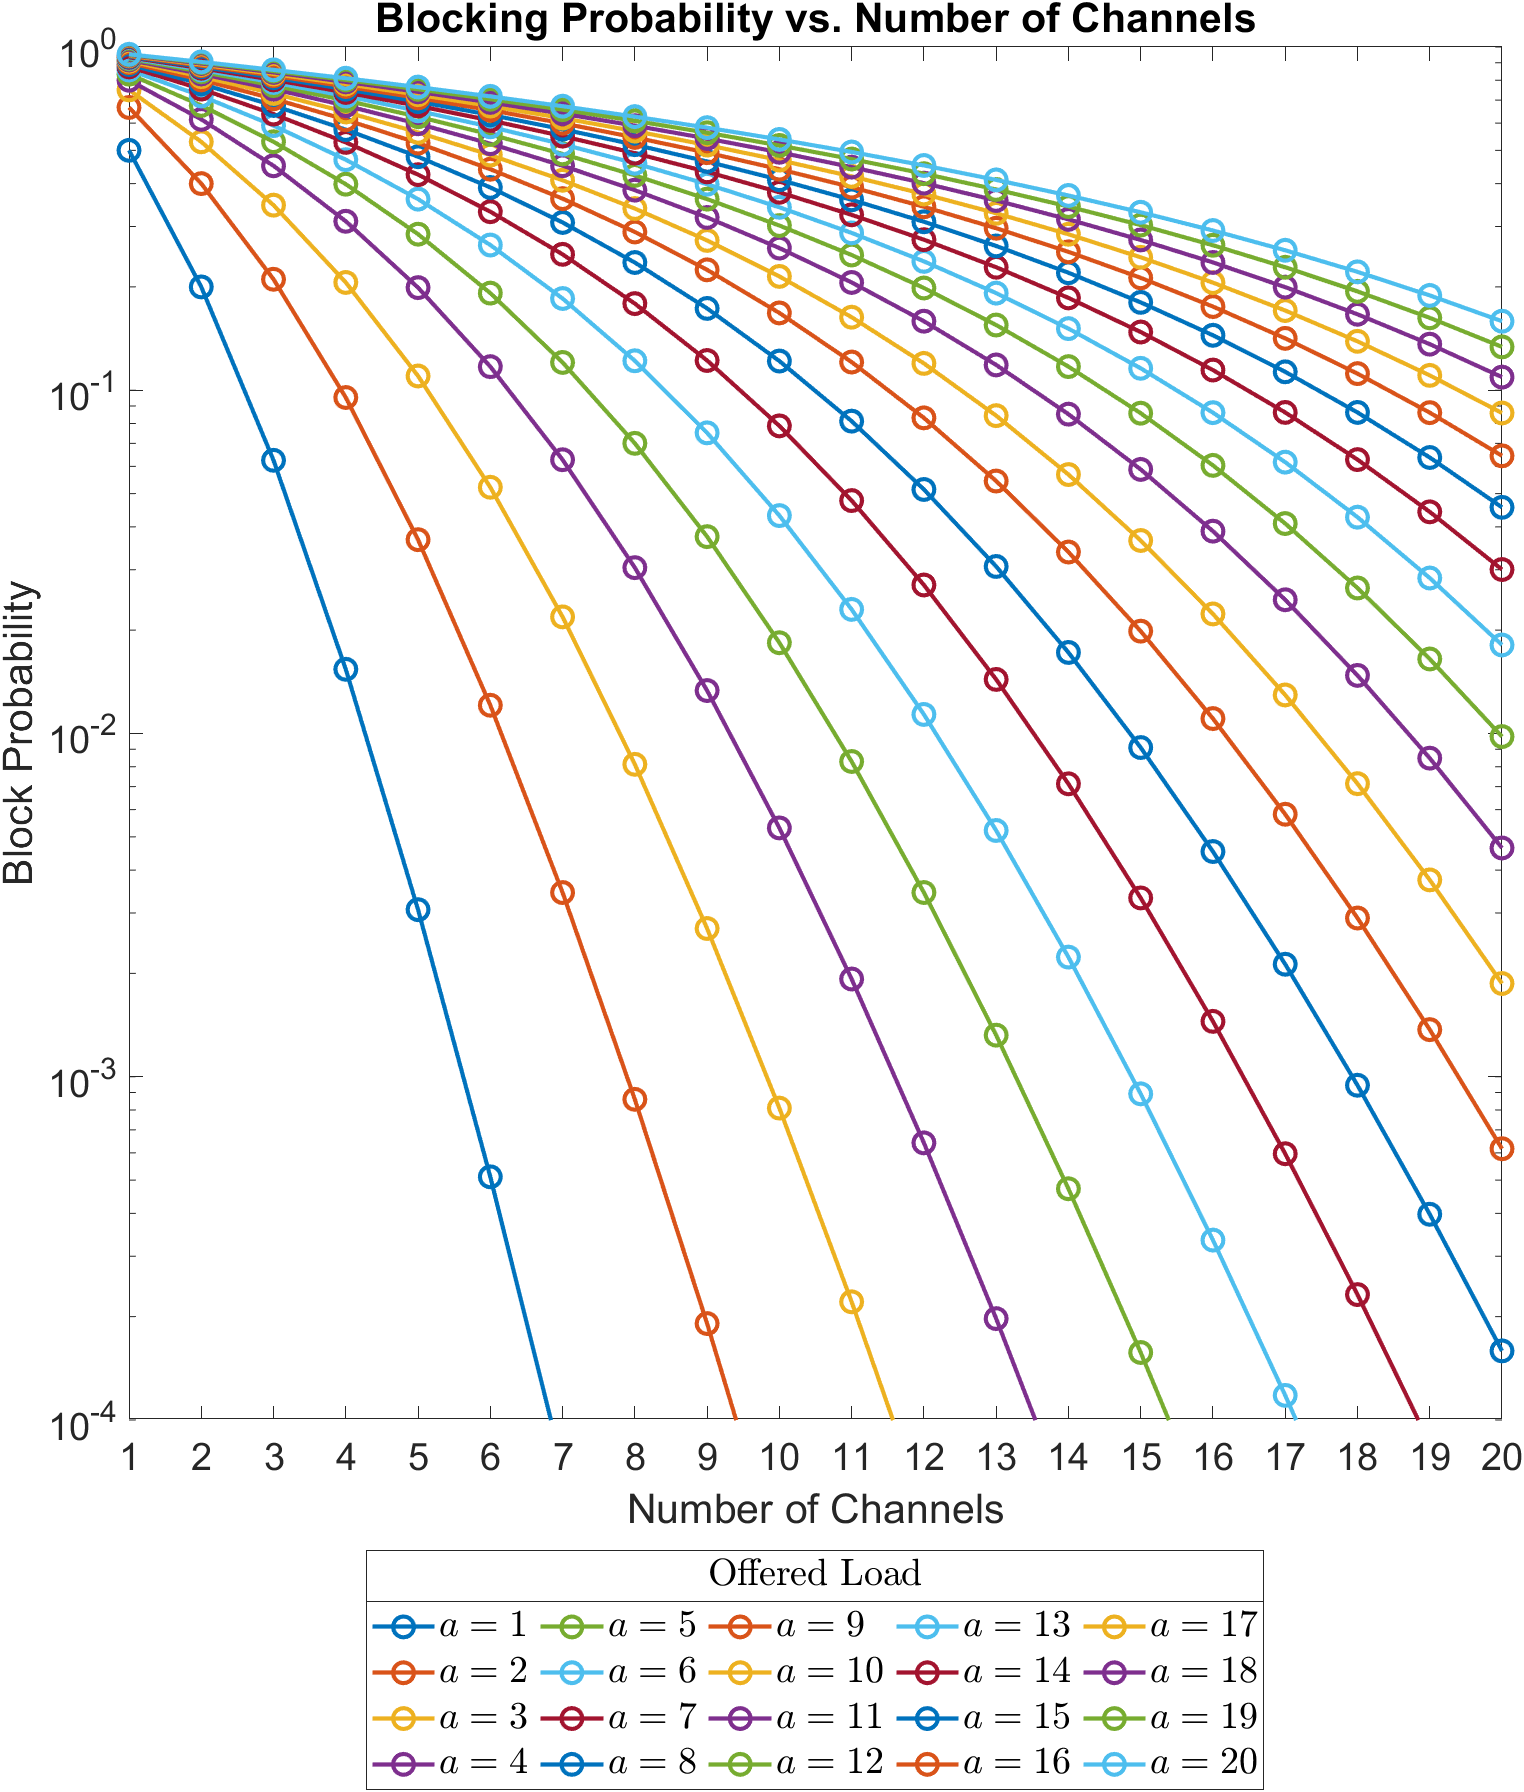
\includegraphics[width=\textwidth]{exp2.png}
\caption{Experiment 2: MATLAB}
\label{fig:exp2_matlab}
\end{figure}

\section*{Experiment 3}


\section*{Experiment 4}
To simulate this case, the code was modified to add a FIFO queue where calls would be placed on call arrival if all channels are full. This queue would be checked on call departure (the only event that can free up a channel) and place a call from the queue that hasn't hung up into any empty channel. The modifications for call arrivals can be seen in Listing~\ref{list:exp4_arrival} and modifications for call departures can be seen in Listing~\ref{list:exp4_departure}.

The probability of not being served versus offered loading for different values of $w$ and $N$ is shown in Figure~\ref{fig:exp4_prob}. We can see that the waiting probability for a given offered load decreases when the number of channels, $N$, increase, and does not demonstrate a significant change when the mean hang-up time, $w$, changes.

The mean time that customers have to wait on the queue versus offered loading for different values of $w$ and $N$ is shown in Figure~\ref{fig:exp4_delay}. We can see that the mean waiting time for 1 Erlangs of offered load depends on the number of channels, $N$, and will decrease as $N$ increases. As the mean hang-up time, $w$, increases the mean queue wait time increases.

\begin{figure}[htp]
\centering
\captionsetup{justification=centering}
\begin{tikzpicture}
	\begin{axis}
		[
		title = {Waiting Probability vs. Offered Load},
		width = 0.969\textwidth,
		%height = 150,
		xmin = 1, xmax = 20, xtick={1,...,20},
		ymin = 0, ymax = 1,
		ylabel = Probability of Customer Waiting, xlabel = Offered Load (Erlangs),
		xticklabel style={
			/pgf/number format/fixed,
			/pgf/number format/precision=3
		},
		scaled x ticks=false,
		legend pos=north west,
		% legend style={at={(0.5,-0.1)},anchor=north},
		% legend columns=5,
		% legend style={font=\scriptsize}
		% some code for adding points
		%nodes near coords={%
		%\footnotesize
		%$(\pgfmathprintnumber
		%{\pgfkeysvalueof{/data point/x}},
		%\pgfmathprintnumber
		%{\pgfkeysvalueof{/data point/y}})$%
		%},
		]
		% \addlegendimage{empty legend}
		% \addlegendentry{\makebox[0pt][l]{\hspace{1.6cm}Offered Load (Erlangs)}}
		\addplot+ [mark=o, thick] table [y=$w5n5_prob$, x=$off_load$]{./data/exp4.dat};
		\addlegendentry{$w = 5, N = 5$}
		\addplot+ [mark=o, thick] table [y=$w5n10_prob$, x=$off_load$]{./data/exp4.dat};
		\addlegendentry{$w = 5, N = 10$}
		\addplot+ [mark=o, thick] table [y=$w10n5_prob$, x=$off_load$]{./data/exp4.dat};
		\addlegendentry{$w = 10, N = 5$}
		\addplot+ [mark=o, thick] table [y=$w10n10_prob$, x=$off_load$]{./data/exp4.dat};
		\addlegendentry{$w = 10, N = 10$}
	\end{axis}
\end{tikzpicture}
\caption{Experiment 4: Waiting Probability}
\label{fig:exp4_prob}
\end{figure}

\begin{figure}[htp]
\centering
\captionsetup{justification=centering}
\begin{tikzpicture}
	\begin{axis}
		[
		title = {Mean Waiting Time in Queue vs. Offered Load},
		width = 0.969\textwidth,
		%height = 150,
		xmin = 1, xmax = 20, xtick={1,...,20},
		ymin = 0, ymax = 450,
		ylabel = Mean Queue Wait Time (seconds), xlabel = Offered Load (Erlangs),
		xticklabel style={
			/pgf/number format/fixed,
			/pgf/number format/precision=3
		},
		scaled x ticks=false,
		legend pos=north west,
		% legend style={at={(0.5,-0.1)},anchor=north},
		% legend columns=5,
		% legend style={font=\scriptsize}
		% some code for adding points
		%nodes near coords={%
		%\footnotesize
		%$(\pgfmathprintnumber
		%{\pgfkeysvalueof{/data point/x}},
		%\pgfmathprintnumber
		%{\pgfkeysvalueof{/data point/y}})$%
		%},
		]
		% \addlegendimage{empty legend}
		% \addlegendentry{\makebox[0pt][l]{\hspace{1.6cm}Offered Load (Erlangs)}}
		\addplot+ [mark=o, thick] table [y=$w5n5_mean$, x=$off_load$]{./data/exp4.dat};
		\addlegendentry{$w = 5, N = 5$}
		\addplot+ [mark=o, thick] table [y=$w5n10_mean$, x=$off_load$]{./data/exp4.dat};
		\addlegendentry{$w = 5, N = 10$}
		\addplot+ [mark=o, thick] table [y=$w10n5_mean$, x=$off_load$]{./data/exp4.dat};
		\addlegendentry{$w = 10, N = 5$}
		\addplot+ [mark=o, thick] table [y=$w10n10_mean$, x=$off_load$]{./data/exp4.dat};
		\addlegendentry{$w = 10, N = 10$}
	\end{axis}
\end{tikzpicture}
\caption{Experiment 4: Mean Delay}
\label{fig:exp4_delay}
\end{figure}
% \clearpage

\begin{lstlisting}[float,language=c,caption=Wait on Call Arrival, label=list:exp4_arrival]
} else {
	/* No free channel was found. The call is placed in queue. */
	fifoqueue_put(sim_data->buffer, (void *) new_call);
	sim_data->waited_call_count++;
}
\end{lstlisting}
	
\begin{lstlisting}[float,language=c,caption=Connect or Hang Up on Call Departure, label=list:exp4_departure]
if ((free_channel = get_free_channel(simulation_run)) != NULL) {
	int queue_size;
	if ((queue_size = fifoqueue_size(sim_data->buffer)) > 0) {
		for (int i = 0; i < queue_size; ++i) {
			new_call = (Call_Ptr) fifoqueue_get(sim_data->buffer);

			if (new_call->hang_up_time < now) {
				sim_data->call_hung_up_count++;
				sim_data->accumulated_queue_wait_time += new_call->hang_up_time - new_call->arrive_time;
				xfree((void *) new_call);
				new_call = NULL;
				continue;
			}

			sim_data->accumulated_queue_wait_time += now - new_call->arrive_time;
			break;
		}

		// If the queue only contained customers that have hung up, we have nothing to do
		if (new_call == NULL) {
			return;
		}

		new_call->arrive_time = now;
		new_call->call_duration = get_call_duration();

		/* Place the call in the free channel and schedule its departure. */
		server_put(free_channel, (void *) new_call);
		new_call->channel = free_channel;

		schedule_end_call_on_channel_event(simulation_run, now + new_call->call_duration, (void *) free_channel);
	}
}
\end{lstlisting}

% \section*{Experiment 5}
To simulate this case, the code was modified to add a FIFO queue where calls would be placed on call arrival if all channels are full. This queue would be checked on call departure (the only event that can free up a channel) and place a call from the queue into any empty channel if the queue contains a call. The modifications for call arrivals can be seen in Listing~\ref{list:exp4_arrival} and modifications for call departures can be seen in Listing~\ref{list:exp4_departure}. The values for $P_w$, $T_w$, $W(1 \text{min})$ were found in simulation and calculated with the given formulas for the following cases:
\begin{enumerate}
\item
$\lambda = 2$, $h = 3$, $N = 10$\\
Simulation results: $P_w = 0.1006$, $T_w = 0.0746$ min, $W(1 \text{min}) = 0.9739$\\
Calculated value: $P_w = 0.0974$, $T_w = 0.0730$ min, $W(1 \text{min}) = 0.9743$

\item
$\lambda = 7$, $h = 2$, $N = 15$\\
Simulation results: $P_w = 0.7198$, $T_w = 1.4224$ min, $W(1 \text{min}) = 0.5662$\\
Calculated value: $P_w = 0.6891$, $T_w = 1.3783$ min, $W(1 \text{min}) = 0.5820$

\item 
$\lambda = 2$, $h = 7$, $N = 15$\\
Simulation results: $P_w = 0.7198$, $T_w = 4.9785$ min, $W(1 \text{min}) = 0.3774$\\
Calculated value: $P_w = 0.6891$, $T_w = 4.8239$ min, $W(1 \text{min}) = 0.4026$
\end{enumerate}

\begin{lstlisting}[language=c,caption=Wait on Call Arrival, label=list:exp4_arrival]
} else {
	/* No free channel was found. The call is placed in queue. */
	fifoqueue_put(sim_data->buffer, (void *) new_call);
	sim_data->waited_call_count++;
}
\end{lstlisting}

\begin{lstlisting}[language=c,caption=Wait on Call Departure, label=list:exp4_departure]
// See if there is are calls waiting in the buffer and there is a free channel. If so, take the next one out and connect it immediately.
if ((fifoqueue_size(sim_data->buffer) > 0) && ((free_channel = get_free_channel(simulation_run)) != NULL)) {
	next_call = (Call_Ptr) fifoqueue_get(sim_data->buffer);

	next_call->call_duration = get_call_duration();
	next_call->waiting_time = now - next_call->arrive_time;

	/* Place the call in the free channel and schedule its departure. */
	server_put(free_channel, (void*) next_call);
	next_call->channel = free_channel;

	schedule_end_call_on_channel_event(simulation_run,
					now + next_call->call_duration,
					(void *) free_channel);
}
\end{lstlisting}

% \section*{Experiment 6}


\end{document}